%! suppress = LineBreak
%! suppress = Unicode
%! suppress = MissingLabel
%! suppress = MissingImport
%! suppress = FileNotFound
\documentclass[../main.tex]{subfiles}

\begin{document}

    \subsection{Testowanie eksploracyjne}

    \begin{table}[H]
        \begin{center}
            \begin{tabular}{p{8cm} p{8cm}}
                \begin{itemize}
                    \item Technika polegająca na jednoczesnym uczeniu się, obserwowaniu
                    oprogramowania, projektowaniu testów i ich wykonywaniu.

                    \item \textbf{Każde podejście do testów jest w jakimś stopniu eksploracyjne.}

                    \item \textbf{Efektywność} techniki zależy od \textbf{stopnia posiadanych umiejętności}:
                    \begin{itemize}
                        \item projektowania dobrych testów
                        \item uważnej obserwacji
                        \item krytycznego myślenia
                        \item kreatywności
                        \item używania praktycznych narzędzi i technik
                    \end{itemize}
                    W eksploracji można używać \textbf{formalnych technik} projektowania testów!
                \end{itemize}
                &
                \textbf{Idea}:
                \begin{enumerate}
                    \item Pobieżna \textbf{eksploracja} systemu jako całości
                    \item \textbf{Sprawdzenie} modułów
                    \item Szczegółowa \textbf{analiza} dwóch rzeczy w jednym z modułów
                    \item Pogłębiona \textbf{analiza zagadnienia}
                \end{enumerate}
            \end{tabular}
        \end{center}
    \end{table}

    \begin{figure}[H]
        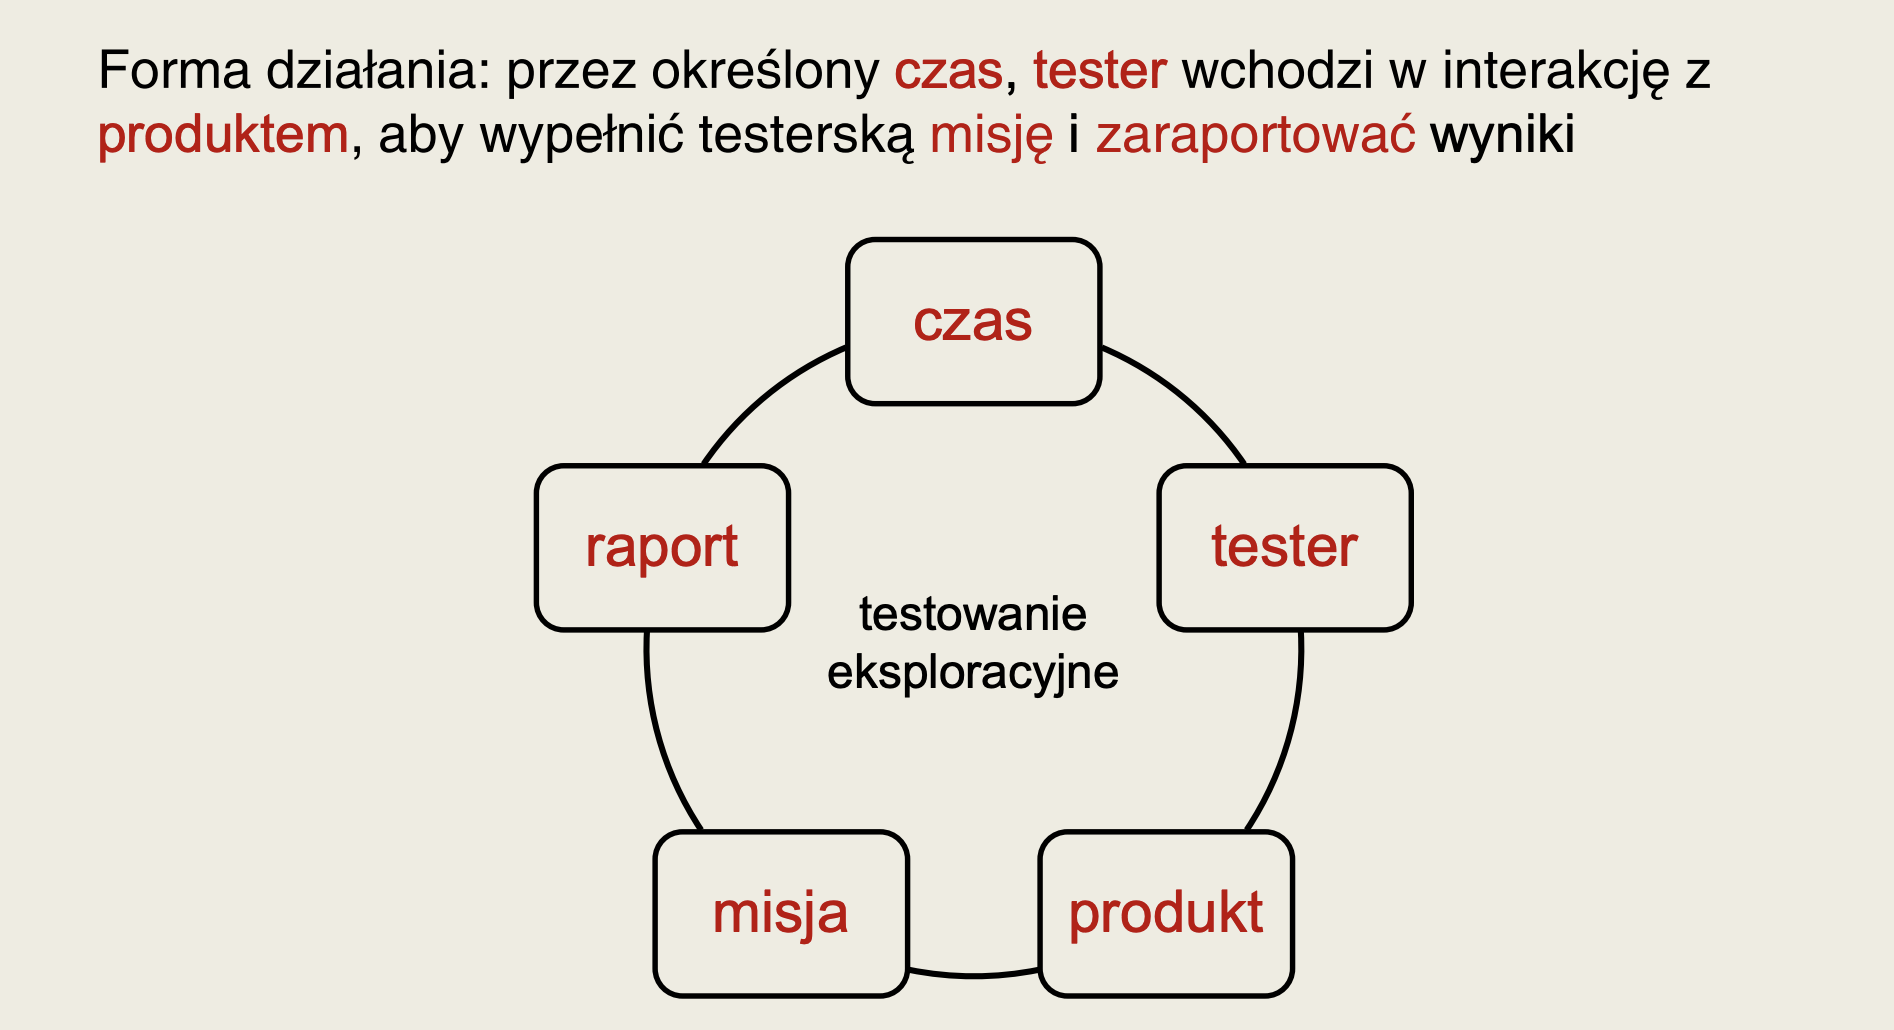
\includegraphics[width=\linewidth]{explore.png}
    \end{figure}

    Przeprowadzane w \textbf{sesjach}, często z użyciem \textbf{karty testów} (test charter):
    \begin{itemize}
        \item np "zidentyfikuj i sprawdź
        wszystkie stwierdzenia z podręcznika użytkownika", "sprawdź GUI pod kątem zgodności ze standardem Windows".
        \item \textbf{nie jest bardzo precyzyjna} – adresatem jest \textbf{tester dobrze znający system}, środowisko,
        słownictwo itp.
        \item daje \textbf{swobodę} i \textbf{nie narzuca} konkretnych \textbf{rozwiązań} i podejść – wiele zależy od samego testera.
    \end{itemize}

    \begin{table}[H]
        \begin{center}
            \begin{tabular}{p{8cm} p{8cm}}
                \multicolumn{2}{c}{\textbf{Kiedy używać testowania eksploracyjnego?}} \\
                \multicolumn{2}{c}{Zwykle zawsze, gdy nie wiadomo jaki ma być następny test.} \\
                \begin{itemize}
                    \item gdy trzeba dać szybką informację zwrotną o nowym produkcie/cesze
                    \item gdy trzeba szybko nauczyć się nowego produktu
                    \item gdy użyto planowego testowania i szukamy różnorodności w testach
                    \item gdy chcemy znaleźć najważniejszy defekt w najkrótszym czasie
                \end{itemize}
                &
                \begin{itemize}
                    \item gdy chcemy sprawdzić pracę innego testera przez niezależną analizę
                    \item gdy chcemy zbadać i wyizolować konkretny defekt
                    \item gdy chcemy określić poziom konkretnego ryzyka w celu oceny zastosowania planowanego testowania w tym obszarze
                \end{itemize}
            \end{tabular}
        \end{center}
    \end{table}

    \subsection{Pomniejsze techniki}

    \begin{table}[H]
        \begin{center}
            \begin{tabular}{| p{8cm} | p{8cm} |}
                \hline
                \textbf{Zgadywanie błędów} & \textbf{Testowanie oparte na listach kontrolnych} \\
                \hline
                \begin{itemize}
                    \item ang. error guessing; czasem utożsamiane z \textbf{testowaniem ad-hoc}
                    \item technika niebazująca na żadnym systematycznym podejściu czy technice
                    \item opiera się na \textbf{doświadczeniu testera} w testowaniu
                    \item tester szacuje (zgaduje), w którym miejscu może pojawić się defekt
                    \item często utożsamiana z nieplanowanym, nieukierunkowanym testowaniem, bez zdefiniowanych celów i bez kontroli postępów
                    \item \textbf{generalnie niepolecana}
                \end{itemize}
                &
                \begin{itemize}
                    \item tester korzysta z \textbf{wysokopoziomowej listy elementów do
                    zanalizowania}, sprawdzenia lub zapamiętania
                    \item \textbf{lista kontrolna} (ang. check-list) jest modelem dla testowania
                    \item lista może dotyczyć różnych aspektów, np.:
                    \begin{itemize}
                        \item charakterystyk jakościowych
                        \item standardów GUI
                        \item kluczowych operacji
                        \item standardów kodowania
                    \end{itemize}
                \end{itemize} \\
                \hline
                \hline
                \textbf{Ataki usterkowe}   & \textbf{Techniki oparte na modelach defektów}     \\
                \hline
                \begin{itemize}
                    \item idea: \textbf{atak} na oprogramowanie przez jego \textbf{interfejs}: użytkowy (GUI, API)
                    lub systemowy (system plikowy, interfejs bazodanowy, interfejs OS)
                \end{itemize}
                &
                \begin{itemize}
                    \item \textbf{taksonomia defektów} to system (hierarchicznych) kategorii
                    stworzony jako pomoc w klasyfikowaniu defektów
                \end{itemize} \\
                \hline
            \end{tabular}
        \end{center}
    \end{table}

    \subsection{Testowanie mutacyjne}
    \begin{table}[H]
        \begin{center}
            \begin{tabular}{p{8cm} p{8cm}}
                \begin{itemize}
                    \item metoda \textbf{oparta na składni}
                    \item można ją zaklasyfikować jako \textbf{białoskrzynkową}
                    \item uważana za jedną z \textbf{najmocniejszych} technik testowania
                    \item bezpośrednio \textbf{testuje testy}, nie program
                    \item pośrednio \textbf{zwiększa jakość} program
                    \item \textbf{mutant} = zmodyfikowany kod (musi być kompilowalny)
                    \item mutacje mogą być dokonywane na kodzie lub kodzie pośrednim
                \end{itemize}
                &
                \begin{itemize}
                    \item \textbf{idea: każdy mutant powinien zostać zabity} przez
                    przynajmniej 1 test (tzn. wynik testu na oryginalnym
                    programie powinien być inny niż wynik testu na mutancie)
                    \begin{itemize}
                        \item test zabijający mutanta jest skuteczny (silny)
                        \item niezabity mutant oznacza słabość suity testowej
                    \end{itemize}
                    \item \textbf{pokrycie mutacyjne} = \# zabitych mutantów / \# mutantów
                \end{itemize}
            \end{tabular}
        \end{center}
    \end{table}

    \begin{table}[H]
        \begin{center}
            \begin{tabular}{p{8cm} p{8cm}}
                \textbf{Zalety}
                \begin{itemize}
                    \item \textbf{wysoce zautomatyzowany} proces, wsparcie narzędziowe
                    \item \textbf{tani} we wdrożeniu (praktycznie za darmo)
                    \item jedna z \textbf{najefektywniejszych} technik testowania
                \end{itemize}
                &
                \textbf{Wady}
                \begin{itemize}
                    \item \textbf{wymaga wielu zasobów, czasochłonny}
                    \item efektywność zależy od doboru operatorów mutacyjnych
                    \item problem \textbf{mutantów równoważnych} = mających ten sam efekt, np != i < w warunku pętli
                \end{itemize}
            \end{tabular}
        \end{center}
    \end{table}

    \subsection{Analiza statyczna}
    Analiza statyczna to analiza artefaktów oprogramowania (najczęściej kodu) przeprowadzana bez wykonywania kodu.
    Zwykle wykorzystuje narzędzia.

    \begin{table}[H]
        \begin{center}
            \begin{tabular}{p{8cm} p{8cm}}
                \textbf{Cechy analizy statycznej}
                \begin{itemize}
                    \item \textbf{wczesne wykrywanie} defektów (przed testami dynamicznymi)
                    \item wczesne wykrywanie podejrzanych aspektów kodu lub projektu
                    \item identyfikacja defektów trudnych do wykrycia w testach
                    \item \textbf{wykrywanie zależności i niespójności} w modelach oprogramowania
                    \item zwiększenie \textbf{pielęgnowalności} kodu
                    \item \textbf{zapobieganie defektom}
                \end{itemize}
                &
                \textbf{Przykładowe metody analizy statycznej}
                \begin{itemize}
                    \item analiza złożoności kodu
                    \item parsowanie kodu
                    \item analiza przepływu danych
                    \item grafy wywołań (dla analizy statycznej integracji)
                \end{itemize}
            \end{tabular}
        \end{center}
    \end{table}

    \begin{table}[H]
        \begin{center}
            \begin{tabular}{ p{8cm} p{8cm}}
                \multicolumn{2}{c}{\textbf{Typowe defekty wykrywane przez analizę statyczną}} \\
                \begin{itemize}
                    \item odwołania do niezainicjalizowanej zmiennej
                    \item niespójne interfejsy,
                    \item niewykorzystane zmienne,
                    \item martwy kod,
                    \item brakująca lub błędna logika,
                \end{itemize} &
                \begin{itemize}
                    \item zbyt skomplikowane instrukcje,
                    \item naruszenie standardów kodowania,
                    \item słabe punkty zabezpieczeń,
                    \item naruszenie reguł modelowania, itp.
                \end{itemize}
            \end{tabular}
        \end{center}
    \end{table}

    \subsubsection{Techniki analizy statycznej}
    \begin{itemize}
        \item \textbf{Analiza złożoności}\\
        \textbf{Złożoność cyklomatyczna} (CC, McCabe cyclomatic complexity) to miara stopnia \textbf{skomplikowania struktury kodu}.

        Metody (równoważne) obliczenia CC:
        \begin{enumerate}
            \item CC = max liczba ścieżek liniowo niezależnych
            \item CC = E – N + 2
            \item CC = liczba zamkniętych obszarów CFG + 1
            \item CC = liczba decyzji w CFG + 1
            (switch z n>2 liczony jako n–1 decyzji)
        \end{enumerate}
        Generalnie, im mniejsza wartość CC, tym lepiej.

        \item \textbf{Parsowanie kodu} - analiza błędów poprawnych syntaktycznie.
        \item \textbf{Analiza przepływu danych}, np:
        \begin{itemize}
            \item przypisanie nieprawidłowej wartości do zmiennej (typy)
            \item użycie zmiennej przed jej zdefiniowaniem
            \item użycie usuniętej uprzednio zmiennej
            \item redefiniowanie zmiennej przed jej użyciem
        \end{itemize}


        \item \textbf{Graf wywołań}
        \begin{itemize}
            \item \textbf{Graf skierowany}, w którym:
            \begin{itemize}
                \item \textbf{wierzchołki} = jednostki oprogramowania (np. moduły, funkcje itp.)
                \item \textbf{krawędzie} = komunikacja między jednostkami (np. wywołanie)
            \end{itemize}

            \item \textbf{Służy do do:}
            \begin{itemize}
                \item określenia kolejności testów integracyjnych
                \item dolnego oszacowania na liczbę testów integracyjnych
            \end{itemize}

            \item \textbf{W testach integracyjnych} chcemy określić ich kolejność tak, aby:
            \begin{itemize}
                \item nie budować zbyt wielu namiastek/sterownków
                \item gdy nastąpi awaria, łatwo będzie zidentyfikować miejsce defektu
                \item będziemy testować rzeczywiste interakcje (np. faktyczne wywołania)
            \end{itemize}
        \end{itemize}
    \end{itemize}
    \begin{figure}[H]
        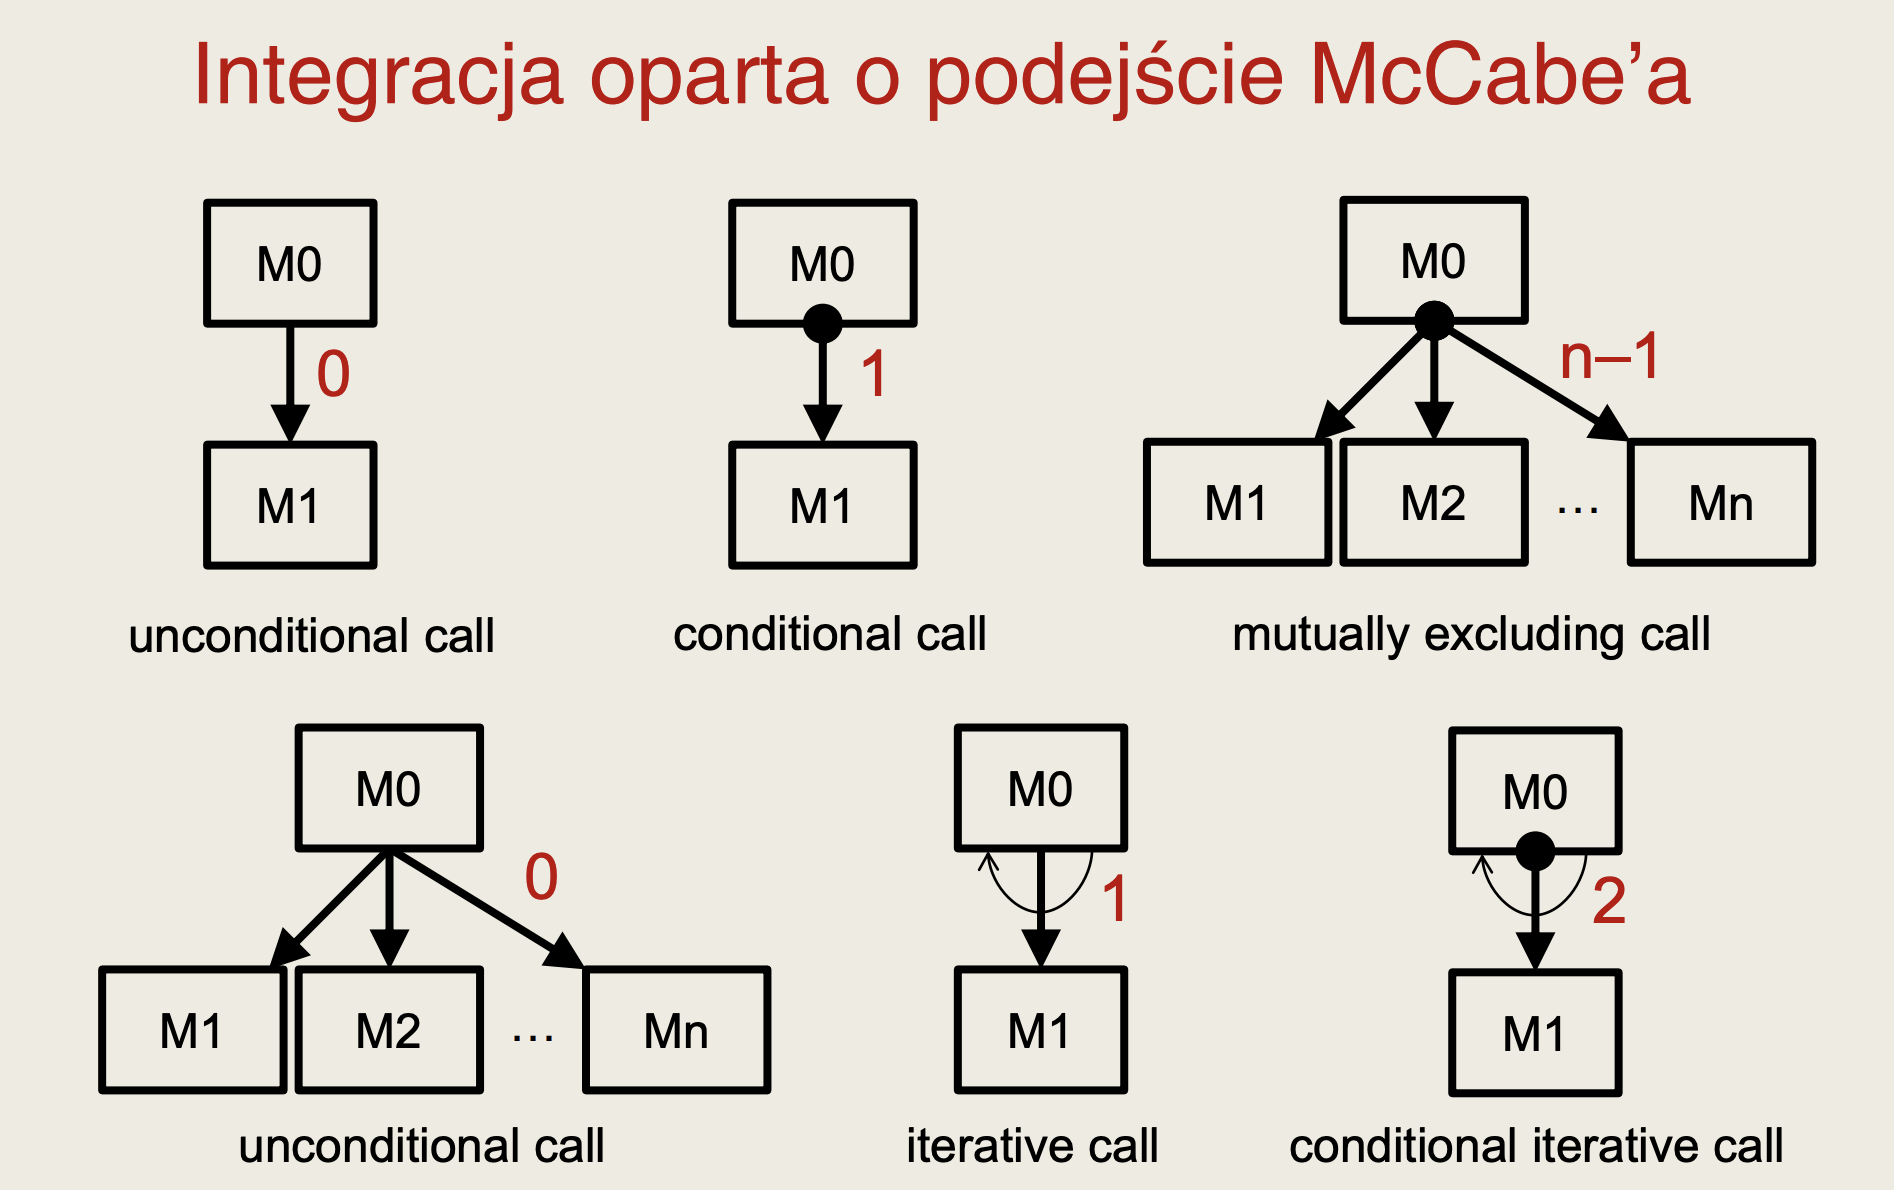
\includegraphics[width=\linewidth]{mccabe.png}
    \end{figure}

    \subsection{Analiza dynamiczna}
    \begin{itemize}
        \item wykorzystywana do \textbf{wykrywania awarii}, gdzie symptomy mogą nie być natychmiastowo widoczne
        \begin{itemize}
            \item np. wycieki pamięci mogą być wykryte w analizie statycznej, ale
            ich wystąpienia będą bardziej czytelne w analizie dynamicznej
        \end{itemize}
        \item analiza dynamiczna \textbf{działa na uruchomionym programie}/systemie
    \end{itemize}

    \subsubsection{Przykładowe techniki analizy dynamicznej}
    \begin{itemize}
        \item \textbf{wykrywanie wycieków pamięci}
        \begin{itemize}
            \item symptomy: stopniowe pogarszanie się wydajności aplikacji
        \end{itemize}
        \item \textbf{wykrywanie dzikich wskaźników}
        \begin{itemize}
            \item program może działać bez zarzutu
            \item program może ulec awarii (crash)
            \item program nie funkcjonuje dobrze (np. brak dostępu do obiektów)
            \item dane w określoym obszarze pamięci mogą być uszkodzone przez wskaźnik i niepoprawnie użyte
        \end{itemize}

        \item \textbf{analiza wydajności}
        \begin{itemize}
            \item narzędzia mogą pomóc wykryć \textbf{wąskie gardła} wydajności
            \item np. informacja o \textbf{ilości wywołań} modułu podczas wykonania
            \item często wywoływane moduły to kandydaci do usprawnienia wydajności
            \item połączona informacja o dynamicznym zachowaniu systemu i o grafach
            wywołań pozwala testerowi zidentyfikować moduły mogące być kandydatami na szczegółowe testowanie
        \end{itemize}

        \item \textbf{analiza zachowania sieci}
        \item \textbf{analiza aplikacji przy użyciu profilera}
    \end{itemize}


\end{document}